\documentclass[tikz,border=3.14mm]{standalone}
\usepackage{amsmath}
\usetikzlibrary{matrix}
\begin{document}
	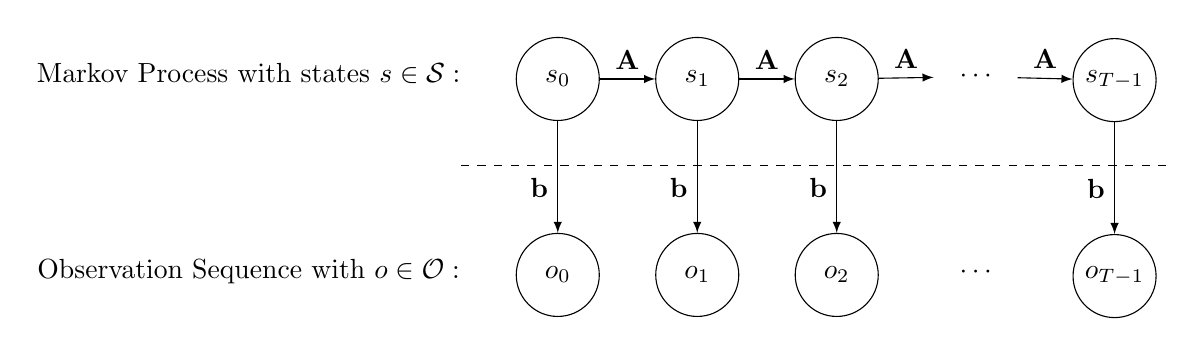
\begin{tikzpicture}
		\matrix [matrix of math nodes,column sep=2em,row sep=4em,cells= {nodes= {circle,draw,minimum width=3em,inner sep=0pt}}, column 1/.style= {nodes= {rectangle,draw=none}}, column 5/.style= {nodes= {rectangle,draw=none}}] (m) {
			\text{Markov Process with states $s \in \mathcal{S}$}: & s_0 & s_1 & s_2 & \cdots & s_{T-1}\\
			\text{Observation Sequence with $o \in \mathcal{O}$}: & o_0 & o_1 & o_2 & \cdots & o_{T-1}\\
		};
		\foreach \X in {2,3,4,5} {
			\draw [-latex] (m-1-\X) -- (m-1-\the\numexpr\X+1) node [midway,above] {$\mathbf{A}$};
			\ifnum\X=5
			\draw [-latex] (m-1-6) -- (m-2-6) node [pos=0.6,left] {$\mathbf{b}$};
			\else
			\draw [-latex] (m-1-\X) -- (m-2-\X) node [pos=0.6,left] {$\mathbf{b}$};
			\fi
		}
		\draw [dashed] ([yshift=1ex]m.east) -- ([yshift=1ex]m.east-|m-1-1.east);
	\end{tikzpicture}
\end{document}